\documentclass[10pt,conference,compsocconf]{IEEEtran}

\usepackage{hyperref}
\usepackage{graphicx}
\usepackage{xcolor}
\usepackage{blindtext, amsmath, comment, subfig, epsfig }
\usepackage{caption}
\usepackage{algorithmic}
\usepackage{cite}
\usepackage[utf8]{inputenc}


\title{CS523 Project 1 Report}
\author{Elvric Trombert, Author 2}
\date{February 2020}

\begin{document}

\maketitle

\begin{abstract}
    Please report your design, implementation details, findings of the first project in this report. \\
    You can add references if necessary. \\
    THE REPORT SHOULD NOT EXCEED 2 PAGES.
\end{abstract}

\section{Introduction}
Give a brief introduction about the project and its aims.

\section{Threat model}
It is important to take into account the main goal of Secure Multiparty Computation is to a set of parties to
interact and compute a joint function of their private inputs while revealing nothing but the
output" \cite{yao}.
Thus our focus here shall be to look at instances where information these private input can be learned by the
adversary which is an information disclosure.
\subsection{Application Structure}
First we need to think about the structure of the application and how information about secret/shares flows through it.

\begin{figure}[ht]
    \centering
    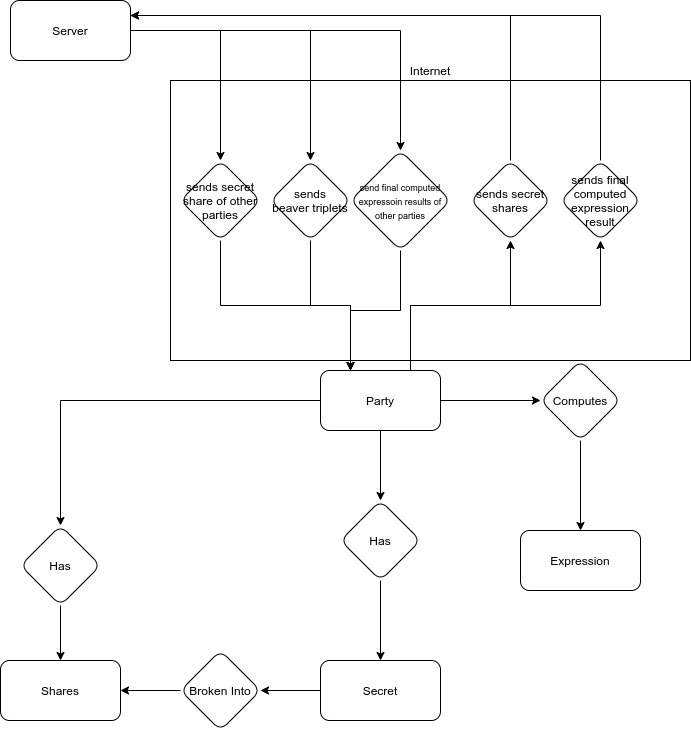
\includegraphics[width=0.5\linewidth]{threat_model.jpg}
    \caption{Dataflow Diagram}
    \label{fig:threat_model}
\end{figure}
\subsection{Attack surface}
From the diagram shown in \ref{fig:threat_model} we can see that there are multiple regions where that can compromise
the confidentiality of the Secret values.
\subsubsection{Compromise on the server side}
Since all shares of secrets are eventually held by the server.
A direct control of the server by an adversary would compromise the confidentiality of all the secrets but could also
compromise the integrity of the secrets and expresion itself.
i.e The adversary could change the value of the secret
shares and even the value of the final computed expression at will.

\subsubsection{Compromise on the Party side}
An adversary that gains control of a party before that said party split its secret into shares will be able
to know the value of that party secrets.
Outside of that stage unless the all parties are compromise it is impossible for the adversary to recover
the value of all the secrets as each party can only access the shares that were destined to it.

\subsubsection{Compromise on the communication route between the parties and the server}
We can see in the dataflow diagram that not all the shares corresponding to a secret are broadcast.
Each party never sends its own share of the secret it owns.
Thus an adversary with network access cannot reconstruct the secrets as they would be lacking one share.


\section{Implementation details}


\section{Performance evaluation}
\subsection{Effect on of the number of parties}
This specific test was run on an expression containing 60 secrets in the form: $s_1 + s_2 + s+_3 \dots s_{30} * s_{31} *
s_{32} * \dots*  s_{60}$
\begin{figure}[ht]
    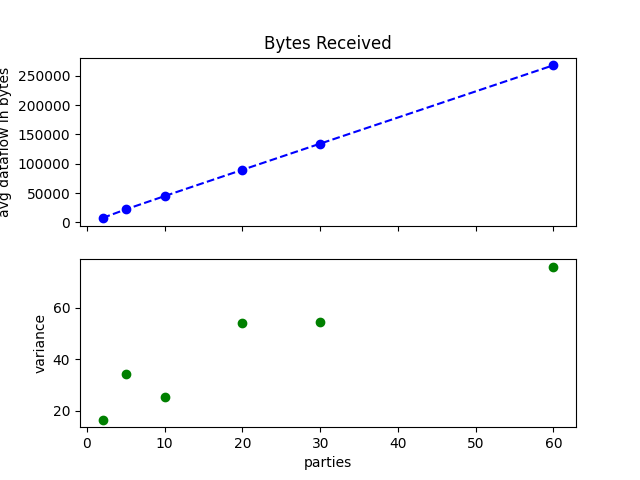
\includegraphics[width=0.49\linewidth]{../performance_analysis/dataflow_in_num_party_change.png}
    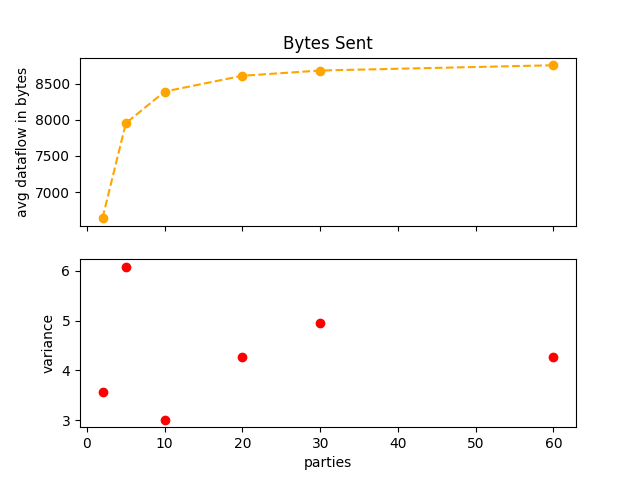
\includegraphics[width=0.49\linewidth]{../performance_analysis/dataflow_out_num_party_change.png}
    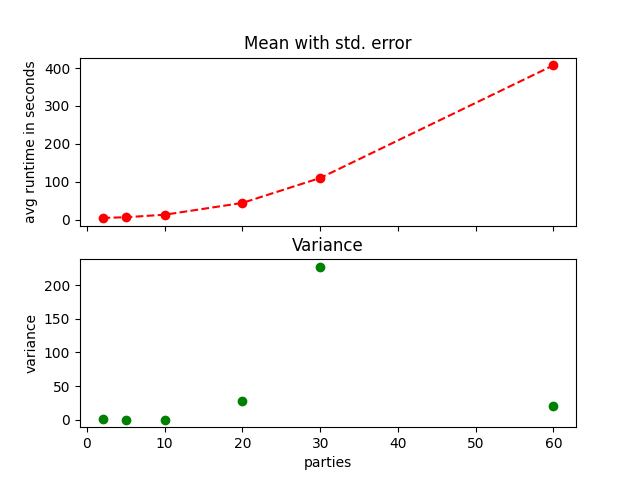
\includegraphics[width=0.49\linewidth]{../performance_analysis/runtime_num_party_change.png}
    \caption{Avg Runtime and Dataflow change based on the number of parties}
\end{figure}
Here

\pagebreak
\subsection{Effect of number of Secret Additions}
Information to write

\begin{figure}[ht]
    \centering
    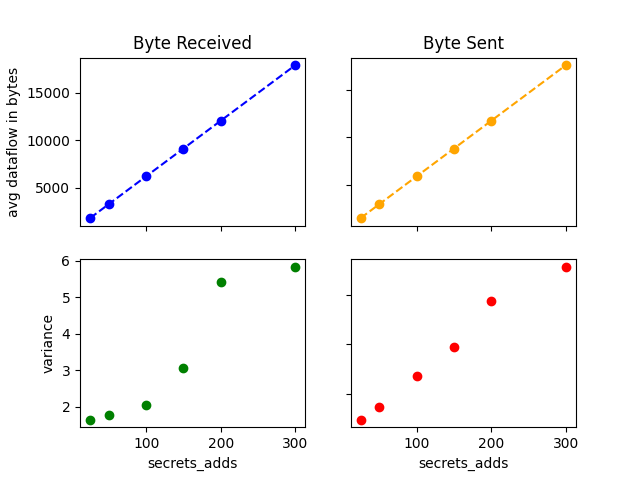
\includegraphics[width=0.49\linewidth]{../performance_analysis/dataflow_secrets_additions.png}
    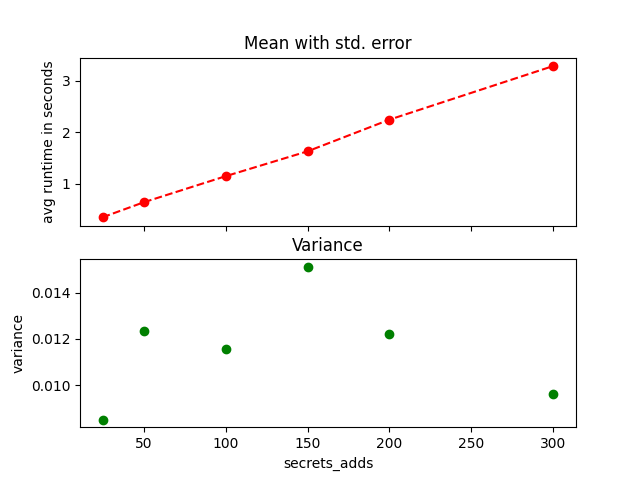
\includegraphics[width=0.49\linewidth]{../performance_analysis/runtime_secrets_additions.png}
    \caption{Avg Runtime and Dataflow change based on the number of Secret Addtions}
\end{figure}

\subsection{Effect of Number of Secret Multiplication}
\begin{figure}[ht]
    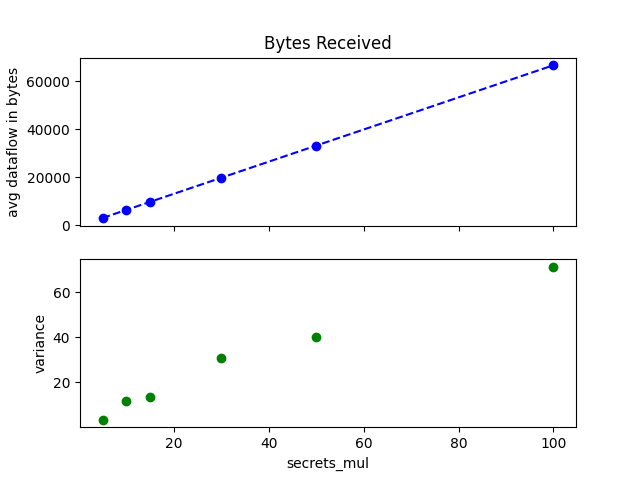
\includegraphics[width=0.49\linewidth]{../performance_analysis/dataflow_in_secrets_multiplications.png}
    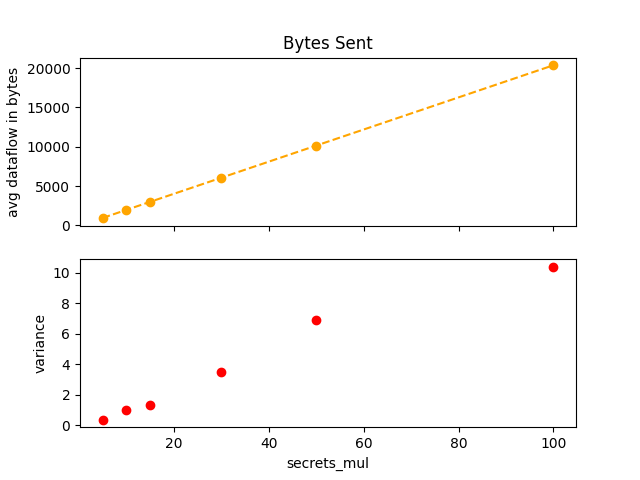
\includegraphics[width=0.49\linewidth]{../performance_analysis/dataflow_out_secrets_multiplications.png}
    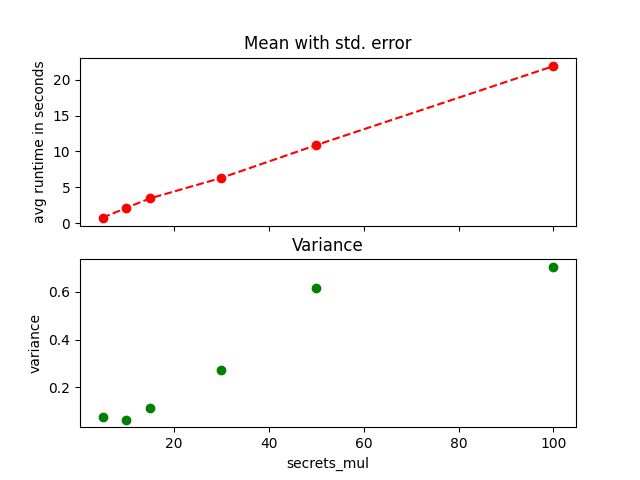
\includegraphics[width=0.49\linewidth]{../performance_analysis/runtime_secrets_multiplications.png}
    \caption{Avg Runtime and Dataflow change based on the number of Secret Multiplications}
\end{figure}

\subsection{Effect of Number of Scalar Addition}

\begin{figure}[ht]
    \centering
    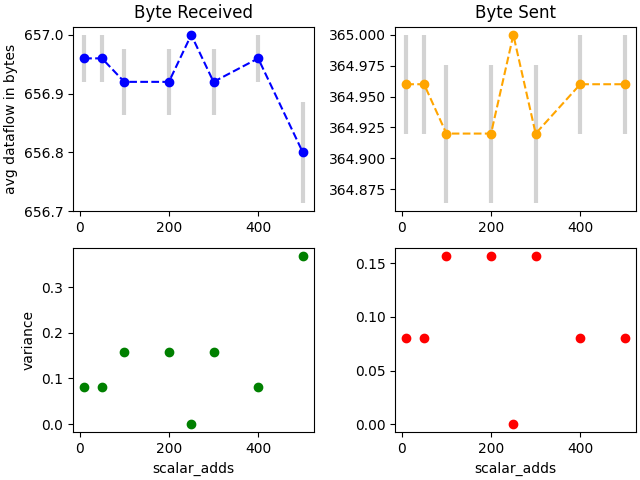
\includegraphics[width=0.49\linewidth]{../performance_analysis/dataflow_scalar_additions.png}
    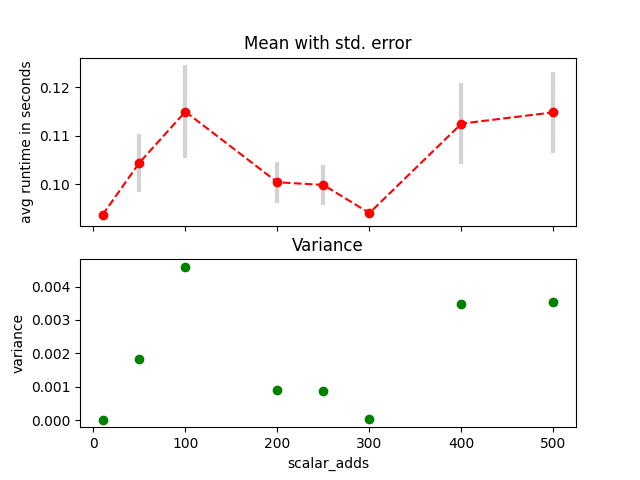
\includegraphics[width=0.49\linewidth]{../performance_analysis/runtime_scalar_additions.png}
    \caption{Avg Runtime and Dataflow change based on the number of Scalar Addtions}
\end{figure}

\subsection{Effect of Number of Scalar Multiplication}

\begin{figure}[ht]
    \centering
    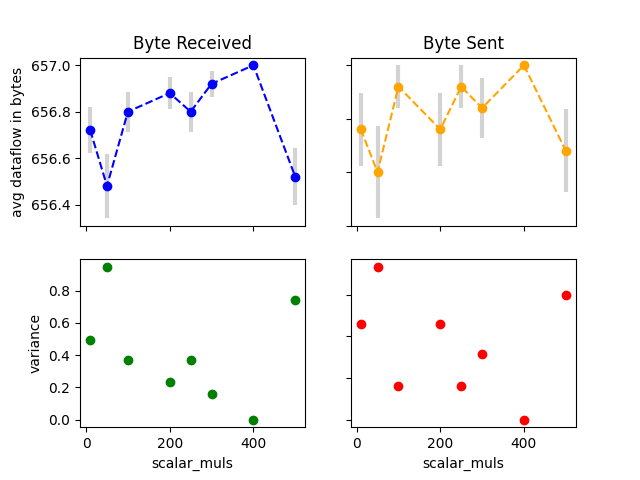
\includegraphics[width=0.49\linewidth]{../performance_analysis/dataflow_scalar_multiplications.png}
    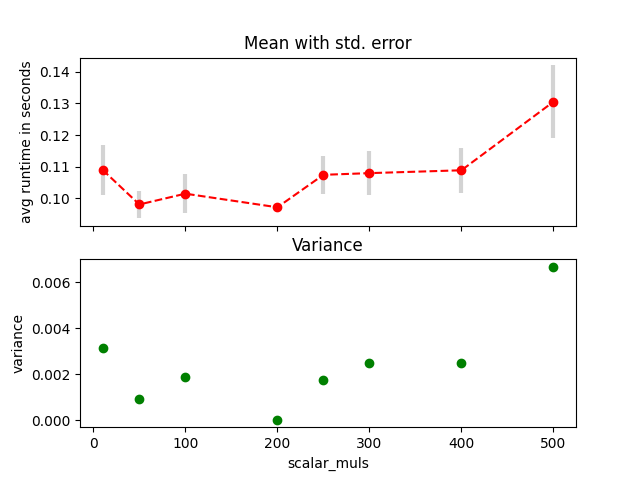
\includegraphics[width=0.49\linewidth]{../performance_analysis/runtime_scalar_multiplications.png}
    \caption{Avg Runtime and Dataflow change based on the number of Scalar Multiplications}
\end{figure}



\section{Application}
Detail the use case of SMC and a circuit for this use case. Discuss possible privacy leakage not
covered by SMC. Discuss a mitigation if needed.

\bibliographystyle{IEEEtran}
\bibliography{bib}
\end{document}
